\documentclass[11pt]{article}
\usepackage[margin  = 1in]{geometry}
\usepackage{hyperref}
\usepackage{amsmath} 
\usepackage{graphicx}
\usepackage{float}
\usepackage{subcaption}
\bibliographystyle{naturemag}
\usepackage{fancyhdr}

\pagestyle{fancy}
\fancyhf{}
\rhead{DRAFT MANUSCRIPT (1 July 2022)}
\lhead{Neronha et al. (2022)}

\begin{document}

%\title{Optimization of Terahertz Leaky Wave Antennas Using Neural Network Modeled Periodically Modulated Slots}
\title{Deep Learning Predictions of Antenna Geometry for Desired Far-Field Signals in Terahertz Leaky Wave Antennas}
\author{Joshua Neronha, Hichem Guerboukha, and Daniel Mittleman \\ \\ \small School of Engineering, Brown University, Providence, RI 02912}
\date{}

\maketitle

\section*{Introduction}

The predictive power of neural networks and machine learning techniques more generally have been applied to a vast array problems ever since the neural network was proposed as a computational technique loosely modeling the brain in the mid-twentieth century. \cite{McCulloch:1943vq} This, of course, includes communications technology -- neural networks have been used extensively in the field because of their unique ability to approximate accurate solutions to nonlinear problems that are commonplace in antenna design. Machine learning models are particularly useful in situations where an analytical solution cannot be obtained and/or numerical simulations are expensive \cite{Kim, Massa}. These types of problems are usually split into two cases, forward and inverse problems. The former refers to situations where models attempt to generate the electromagnetic response given some parametric input, while the latter attempts the reverse: predicting those parameters given some signal \cite{9395365}. \\

\noindent Examples of direct problems include approximating an antenna's output given a geometry \cite{8608745} or modeling a metasurface \cite{Nadell:19}, which could take a finite-element model hours or longer to solve, limiting real-time simulation and design. Inverse problem considers the opposite direction, for example reconstructing an image from scattered light \cite{Sun:18}. There have been many applications of neural networks to communications-related problems, for example, in the optimization of massive multiple-input multiple-output (MIMO) systems to improve signal reconstruction quality \cite{8322184}, physical layer design \cite{DBLP:journals/corr/OSheaEC17}, or predicting channel state information \cite{8395053}. Neural networks and deep learning are particularly useful and interesting in communications applications because of their strength in predicting complex, nonlinear, and multivariate relationships that underly electromagnetics \cite{raissi2018deep}.\\

\noindent We are particularly interested in the inverse problem of terahertz leaky-wave antenna (LWA) design because of its high applicability to the field of communications -- given some arbitrarily desired far-field pattern, how can we quickly design, fabricate, and test an antenna that meets our needs? Periodic leaky wave-antennas are especially interesting for signal design because of their characteristic emissions at various angles, both forward and backwards scattering, that depend on the periodicity, allowing for a wide variety of potential peak angles \cite{6556051}. And while traditional communications systems demand broad angular emission, the terahertz range (i.e. $>$ 100 GHz) requires focusing power along narrow directional beams due to substantial power loss as a result of free path losses at higher frequencies \cite{doi:10.1063/1.5014037, Ghasempour:2020tz}, meaning that highly specific peak profile design is crucial. \\

\noindent LWAs are simple metallic waveguides that have proven very effective in the terahertz range and are particularly interesting because they emit radiation at a frequency-dependent angle with a one-to-one relationship between frequency and angle, which is quite valuable given the narrow character of beams in the terahertz range. \cite{doi:10.1063/5.0033126} They have been used in a number of diverse applications including link discovery \cite{Ghasempour:2020tz}, multiplexing and demultiplexing \cite{Karl:2015uh, Ma:2017vo}, and for radar and object detection purposes \cite{Amarasinghe:20, Amarasinghe:21}. Leaky-wave antennas also stand out for our purposes of rapid design and experimentation because of the ease of fabricating them using hot-stamping techniques \cite{Guerboukha:21}. This inverse problem has been explored in the terahertz range using deep neural networks in the context of designing structures to obtain an optimized geometry that produces the desired signal, particularly in relation to metasurface design \cite{Deng:21, 9602997}. The inverse Leaky-wave antenna problem has also been explored, but using a genetic algorithm and outside of the terahertz range at much higher frequencies \cite{Jafar-Zanjani:2018vy}. \\

\noindent As a result, in this paper, we propose a model to predict the ideal LWA geometry that will generate desired far-field radiation in the terahertz range. Specifically, we suggest an antenna design where a LWA is broken into sub-slots, each of which can either be metallic, transparent, or somewhere in between (i.e. partially transparent). Thus, we find that any slot composed of an array of these sub-slots forms a linear superpositioning of periodic modes that can be used to generate highly specific peak profiles. We use the hot-stamping technique to rapidly prototype and test antennas in the field and view the predictive model as a natural counterpart to rapid prototyping methods.

\section*{Methods}

There are two components to the methodology of this investigation: the computational methods used to construct the model, and the experimental methods applied to confirm the model's validity.

\subsection*{Computational Methods}

We consider a LWA based on a parallel plate waveguide with plate separation of 1 mm, the fundamental transverse electric (TE$_1$) mode, and a frequency of 200 GHz. Instead of a uniform 1D slot \cite{doi:10.1063/5.0033126}, we discretize the slot into 36 0.5-mm sub-slots which can be modulated in their transparency. This approach is similar to the approach taken in past explorations of metasurface design \cite{Liu:2022tg, Jafar-Zanjani:2018vy}. According to Floquet theory \cite{6556051}, a periodic array of slots excites an infinite number of space harmonics each with its distinct dispersion constant $\beta_p$:

\[\beta_p=\sqrt{k_0^2 - (\frac{\pi}{h})^2} +\frac{2\pi p}{\Lambda} \tag{1}\] 


\noindent where $k_0$ is the free space wave number, $h$ is the plate separation, and $\Lambda$ is the slot periodicity. Each different mode peaks at some given angle $\theta$ defined by $\theta=\cos^{-1}(\beta_p/k_0)$, given that the excited modes can be consider fast-wave (i.e. $|\beta_p|>k_0$ ) \cite{6556051}. Our primary objective is to generate multiple beams with specific magnitudes at specific locations, which we demonstrate in Figure 2a using numerical simulations of four periodic waveguides with different periodicities. Each different period has peaks at different angles. Therefore, instead of a periodic geometry, we consider a non-uniformly periodic array of slots in order to exploit multiple periodicities and thus excite multiple modes, producing peaks at multiple angles. By Fourier decomposition, we note that any non-periodic slot design can be viewed as a linear combination of periodic designs $\beta_p$, each peaking at an angle $\cos(\theta)=\beta_p/k_0$. The strength (amplitude) of individual peaks can be related to the Fourier coefficients of this decomposition. Our discretized geometry imposes limits on the possible excited Floquet modes, by constraining the values of $\Lambda$. Indeed, due to the discretization, the possible $\Lambda$ for a total slot length $\ell$ and sub-slot length $\xi$ given by:

%this equation, honestly, I essentially came up with myself. I'm not sure if someone else has derived this equation, I couldn't find it anywhere. If you can't please give it a sanity check lol

\[(\Lambda_k)^{\frac{\ell}{4\xi}}_{k=1}, \textrm{where } \Lambda_k=2k\xi \tag{2}\]

\noindent Furthermore, due to the fast-wave requirement (i.e. $|\beta_p|>k_0$), only a few select modes will be able to leak out of the waveguide, meaning that for a given geometry only some of the  peaks will be present. A schematic of the proposed scheme, in which each sub-slot can either be transparent or metallic, is shown in Figure 1a. For a given geometry, we can calculate all of the possible Floquet peaks by calculating $\beta_p$ for each possible spatial mode for each possible periodicities in this geometry, ranging from $\Lambda$ = 1mm (i.e. 1 transparent, then 1 metallic, etc.) to $\Lambda$ = 9mm (i.e. 18 transparent slots and 18 metallic slots). We calculate the angles for only those modes that satisfy the fast-wave requirement for this geometry in order to find all possible Floquet peaks, which we plot in Figure 2b -- note that there are almost sixty possible peaks!

\begin{figure}
		\centering
		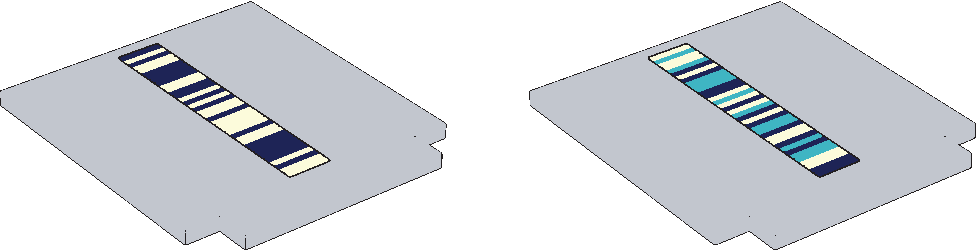
\includegraphics[width = 6in]{figures/fig5pdf}
		\caption{Leaky wave antenna geometry. The antenna is a simple parallel-plate waveguide with non-uniformly periodic sub-slots. a) The binary case, where dark sub-slots represent transparency and light sub-slots represent opaqueness. b) The grey case, when in addition to transparent and metallic sub-slots, there are also partially transparent slots.}
\end{figure}


\begin{figure}[H]
	\centering
	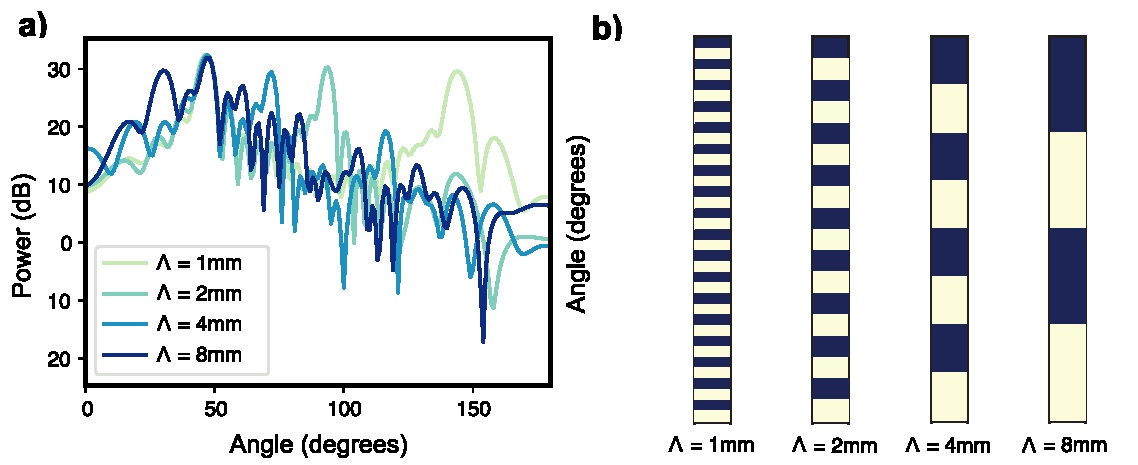
\includegraphics[width=6in]{figures/theorypdfslots}
	%we still have theorypdf.pdf which was that weird scatter plot... do we like that? maybe not the best way to represent but I can't think of a better way.
	\caption{Floquet theory predictions for different geometries of uniform periodicities. a) Numerical simulations for uniformly periodic LWAs with four different values of $\Lambda$; each peaks at different angles, indicating how we use superposition of modes to generate a wide array of possible angles. Note that all periods have a maximum around 48 degrees, which is the primary mode for a LWA of these dimensions. b) The slots used to generate these uniform periodicities; the light sub-slots indicate metal and the darker sub-slots are transparent.}
\end{figure}

\noindent Figure 2 indicates that modulating the periodicity of the geometry we describe enables far-field peak formation at a wide variety of angles, indicating that is a useful regime in which to design a slot based on some desired far-field signal. Solving this inverse problem (i.e. calculating the slot for some given far-field profile), however, is difficult; deriving an analytical expression for a complicated regime is difficult if not impossible, and solving numerically would require iteration through multiple antenna designs until arriving at an optimal solution, essentially searching for one needle in a haystack of $2^{32}$ possible antenna geometries. This is where the idea of a neural network model enters -- deep learning methods are effective at describing nonlinear relationships of complex systems simply by providing training data from which the model can ``learn'' \cite{raissi2018deep}. Thus, we build a model that predicts the slot geometry for some input of a desired far-field signal. \\


\noindent In order to build a model that can predict a slot for a given far-field pattern, we first must generate training data. We build a numerical simulation of a leaky-wave antenna with a slot of length 18 mm divided into 36 sub-slots, each of which is 500 microns in length. The sub-slots are evenly divided between categories (i.e. metallic or transparent). We automate this random geometry generation and simulation using MPh \cite{john_hennig_2022_6312347}, an open-source Python package that enables controlling numerical simulation software using its API. Basic combinatorics theory tells us that there are over 9 billion possible slot designs that can be generated, indicating the usefulness of deep neural networks in this prediction task given the sheer number of possible outputs. Using only a few tens of thousands sets of training data, we will  predict an optimal slot design for an arbitrary peak profile. Each simulation takes approximately one minute to complete, meaning that generating training data is quite slow, but once the model is built it can produce an ideal slot for some far-field pattern in milliseconds, reinforcing its usefulness as a complement to rapid prototyping techniques. \\

\noindent 20,000 instances of COMSOL simulation data were generated as the data source for the deep neural network, with a test-train split of 80-20 \cite{molecules26041111}. The network, which is built with TensorFlow \cite{tensorflow2015-whitepaper}, a popular deep-learning library, has one convolutional layer for feature extraction \cite{albawi2017understanding} connected to six sequential fully-connected layers, each of which have 2000 neurons and use a LeakyReLU activation function with $\alpha = 0.1$ \cite{nair2010rectified}. The model uses the Adam optimizer \cite{kingma2014adam} and has a learning rate of 0.0001, batch size of 128, and trains the model over 35 epochs \cite{smith2018disciplined} and predicts the output of each individual sub-slot with a sigmoid activation function indicating the probability that a given sub-slot should be transparent. The model is visualized in Figure 3. \\

%also I still need to expand on ML techniques at use here...

\begin{figure}[H]
	\centering
	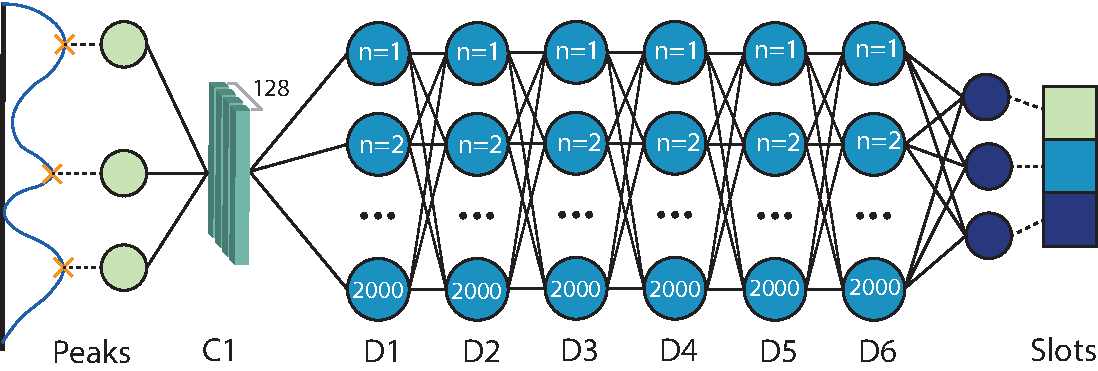
\includegraphics[width=5.2in]{figures/fig1pdf}
	\caption{Neural network architecture schematic. The amplitudes at the angle of each possible Floquet mode are used as the input data and passed through one convolutional layer and six hidden layers within a neural network architecture to predict the  slot design that will yield the closest possible signal. Full network parameters can be found in the code}
\end{figure}

\noindent The tricky part of the inverse problem, as we consider here, is finding an appropriate loss function -- the primary objective is to generate a slot that minimizes the difference in signal compared to what is desired, but in order to use this basis as our loss function, we would need to compute the far-field signal for each new slot we generate as we train the model, which would be extraordinarily (and unfeasibly) computationally expensive. Thus, instead, we turn to the naive idea of making the generated slot look as similar to the given training slot for a given peak profile as possible, although not ideal (one can easily imagine a situation where a slot design was simply offset by 1 in either direction, from which we would expect a very similar response yet would likely score poorly in accuracy). Modified loss functions that introduced a convolutional element in order to emphasize spatial relationships and not exact locations of a sub-slot were tested but performed poorly compared to the naive loss funcrion. Given that this is a binary classification problem for each sub-slot, we use binary cross-entropy (BCE) loss. \cite{10.1145/1102351.1102422} \\

\noindent In addition to modulating between transparent and opaque sub-slots, one can imagine many other possible modulation schemes. While the exploration of these possibilities warrants a paper of their own, we choose to extend our model here to consider the case of partially transparent sub-slots. We generate training data and build a model just as we did with the binary case, with the only difference being that the sub-slots are split between 0\%, 50\%, and 100\% opacity, meaning that there is now an ``in-between" option for sub-slots between metallic and transparent, which we will call the ``grey'' case given the in-between nature of partially transparent sub-slots \\

\subsection*{Experimental Methods}

\noindent We also compare the predictions generated by numerical and machine learning techniques to experimental data. We produce simple hot-stamped leaky-wave antennas \cite{Guerboukha:21} and use a terahertz time-domain spectroscopy (TDS) system to measure the experimental far-field response, scanning both the forward and backwards scattering directions by moving the receiver along a rotation stage. The antenna designs are hot stamped -- meaning that the designs are printed in black and white using a standard laser printer and then passed through a laminator with a sheet of gold foil placed on top, a process that takes only a few minutes and enables rapid prototyping of LWAs. The completed LWA designs are shown in Figure 4a and 4b for both the binary and grey schemas. 

\begin{figure}[H]
	\centering
	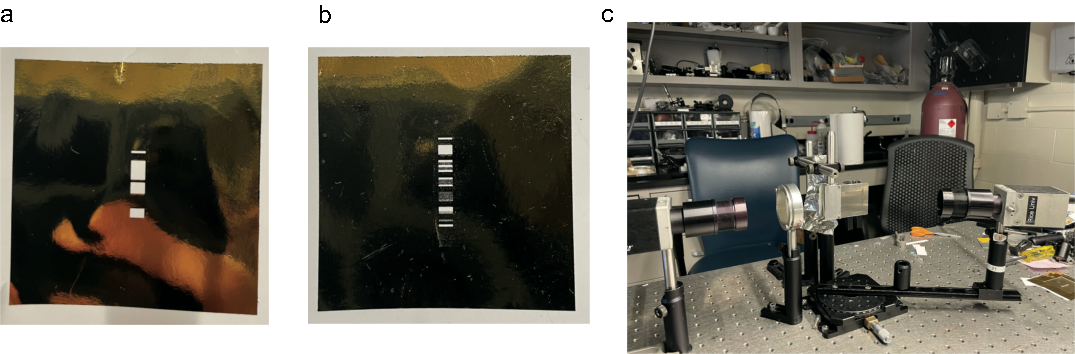
\includegraphics[width=6in]{figures/setuppdf2}
	\caption{a) sample hot-stamped binary antenna; b) sample hot-stamped greyscale antenna; c) experimental setup, where the LWA is mounted on a rotation stage between a transmitter and receiver connected to a terahertz time-domain spectroscopy system}
\end{figure}

\noindent The hot-stamped surfaces are then attached to a metal plate, followed by a 1mm spacer and another plate of metal in order to form a parallel plate waveguide. This rapidly fabricated antenna is then mounted in the center of the rotation stage and aligned with the transmitter, lens, and coupler; the receiver is attached to the rotation stage and is moved to sweep the angular response of the far-field signal.

\section*{Results and Discussion}

\subsection*{Binary Sub-Slot Scheme}

For some given far-field response, the compiled model extracts the Floquet peaks and predicts each individual sub-slot's probability of being transparent (i.e. a value close to 0 indicates the sub-slot should be metal, whereas a value close to 1 indicates a transparent sub-slot) using a sigmoid activation function. In Figure 5, for two random peak profiles inputted into the model, the objective signal and the slot that created it are shown alongside the slot design that the model predicted and the far-field pattern that slot actually generates.

\begin{figure}[H]
	\centering
	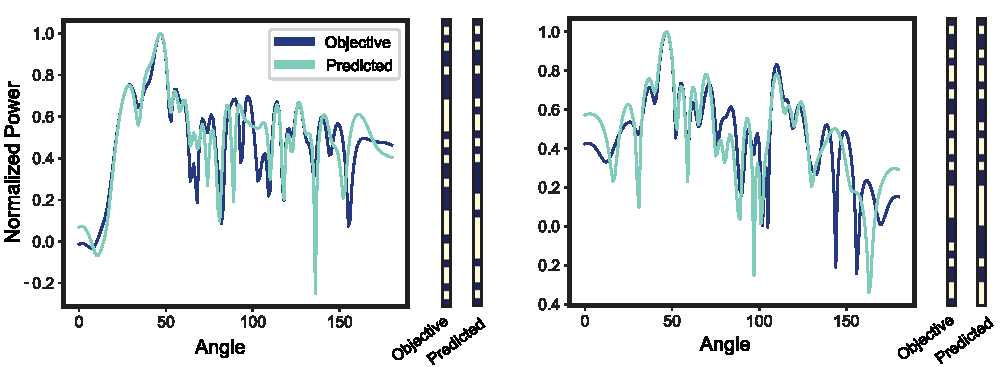
\includegraphics[height=2.4in]{figures/binaryexamples}
	\caption{Model predictions for two different peak profiles. The left slot design is the randomly generated slot used to generate the objective profile and the right slot design is what the model predicted for the objective far-field signal. The numerically-calculated far-field signal generated by the predicted slot is overlaid the objective signal. The MSEs of the left and right examples are 0.0155 and 0.0250, respectively.}
\end{figure}

\noindent However, what determines the usefulness of our model is not the similarity of the slot but the similarity of the signal it generates to the objective. In order to consider the accuracy and usefulness of our model, we use the following procedure:

\begin{enumerate}
	\item Using the testing dataset, extract the Floquet peaks from the far-field signal and pass them through the model to obtain slot geometry predictions
	\item Perform numerical simulation of the predicted slot geometries to obtain their far-field patterns
	\item For each testing sample, compare the far-field response between the objective from the training set and the far-field response from the model-generated slot from Step 2 and compute MSE
\end{enumerate}

\noindent This procedure enables us to measure the performance of the model by a more useful metric than how similar the slot geometry is; rather, we can compare the similarity of the objective far-field response with the far-field response of the slot geometry the model predicts is optimal based on the objective input. Using the mean square error computed in Step 3, we plot a histogram of MSE in Figure 6a and compare it to a control where we compute the MSE between two random signals. The shape of the distribution in Figure 6a matches that of similar work \cite{Nadell:19}. We conduct a two-sided Z-test -- the requirements of which are satisfied given that the histogram indicates a normal distribution, there are 30+ samples, and samples are independent -- and confirm the model's predictive value is statistically significant with a p-value of 2.91e-89, which indicates significance at a very low value of $\alpha$. The average MSE of the model results is 0.0361, and the subslot prediction accuracy is 70.0\%, which is above the baseline value of fifty percent at which there would be no predictive value. 
\begin{figure}[H]
	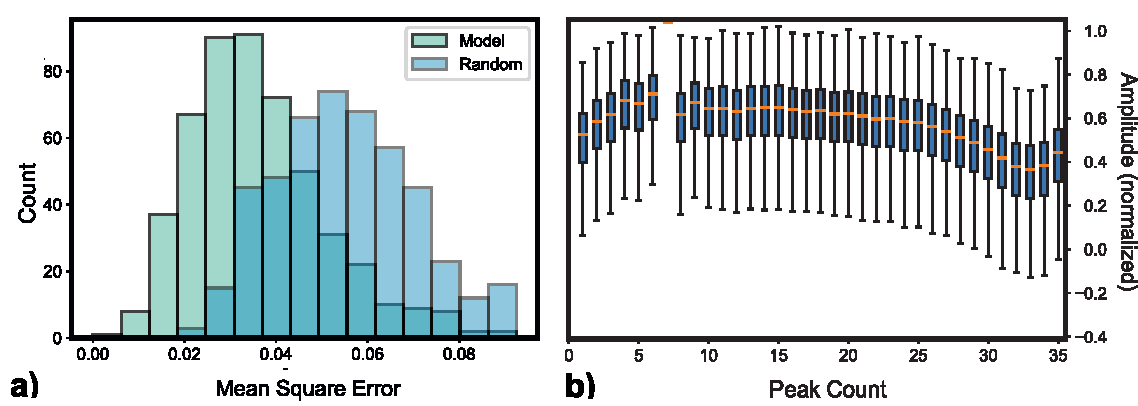
\includegraphics[width=6.5in]{figures/fig6apdf}
		\caption{a) Mean square error (MSE) histogram. The horizontal displacement between the two histograms shows that the model predicts significantly more accurate antenna geometries than the control and is confirmed by a Z-test. b) Box plot of the possible values at each peak. A wide array of values are possible at each peak, indicating that the model may be effective over a wide range of far-field signals.}
\end{figure}

\noindent Figure 6b shows the wide range of normalized far-field power in dB at each possible peaks. The seventh peak, which occurs at 48 degrees, is always the highest because that is the primary mode of an LWA regardless of periodicity. Overall, we see that most Floquet peaks have a wide range of possible values, indicating that our model can be used to predict an ideal geometry for a wide range of far-field patterns. The two examples in Figure 5 showcase the ability of the model to produce reasonable slots that approximate the desired far-field signal. These two cases showcase some of the better performance of the model, and like most models, not all inputs will yield a useful result. However, even for objective signals that yield substantially higher values of mean-square error, the overall peak behavior is often well-preserved, albeit with less exact results and more missed peaks, as would be expected from a higher MSE. Indeed, the goal of this investigation is to demonstrate the usefulness of neural networks for predicting antenna geometry, not to build a perfectly-tuned model. \\

\noindent We also wish to compare our numerical predictions to experimental observations to test if the scheme we discuss is physically plausible for real-world antennas. First, using a terahertz time-domain spectroscopy (TDS), we measure and plot angle versus frequency for two different slots, one with a uniform periodic slot and one with our unique periodically-modulated slots as in Figure 6 below.

\begin{figure}[H]
	\centering
	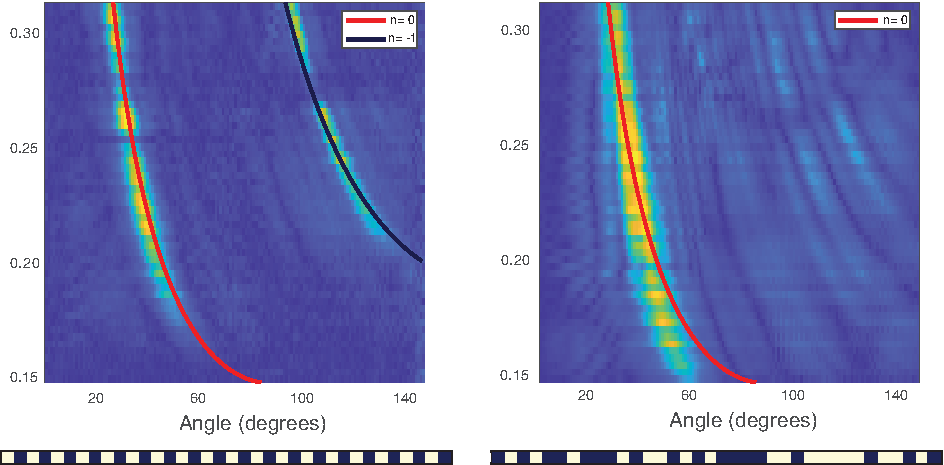
\includegraphics{figures/exp-fig1pdf}
	\caption{Experimental time-domain spectroscopy (TDS) measurements for two different slot designs, the left with only one periodicity and the right with a linear combination of periodicities. In the left panel, we see two discrete modes, whereas in the right panel we see a wide array of lower-power modes, as we would expect from a non-uniformly periodic slot.}
\end{figure}

\noindent Figure 7 confirms our expectations from Floquet theory. For the simple periodic slot, we see the main, non-periodic mode in addition to the one fast-wave Floquet mode. However, at right, we see many Floquet modes at play due to the periodicially-modulated nature of the slot; these two plots pose a sharp contrast to one another and show how our method is capable of producing a multitude of possible slot designs. From the TDS data in the right panel of Figure 7, we extract the far-field signal at 200 GHz and plot against the simulation data (both the objective signal, which is what we want to attain, and the expected signal, which is what we would expect for the slot the model actually predicted) for that slot in Figure 8 below.

\begin{figure}[H]
	\centering
	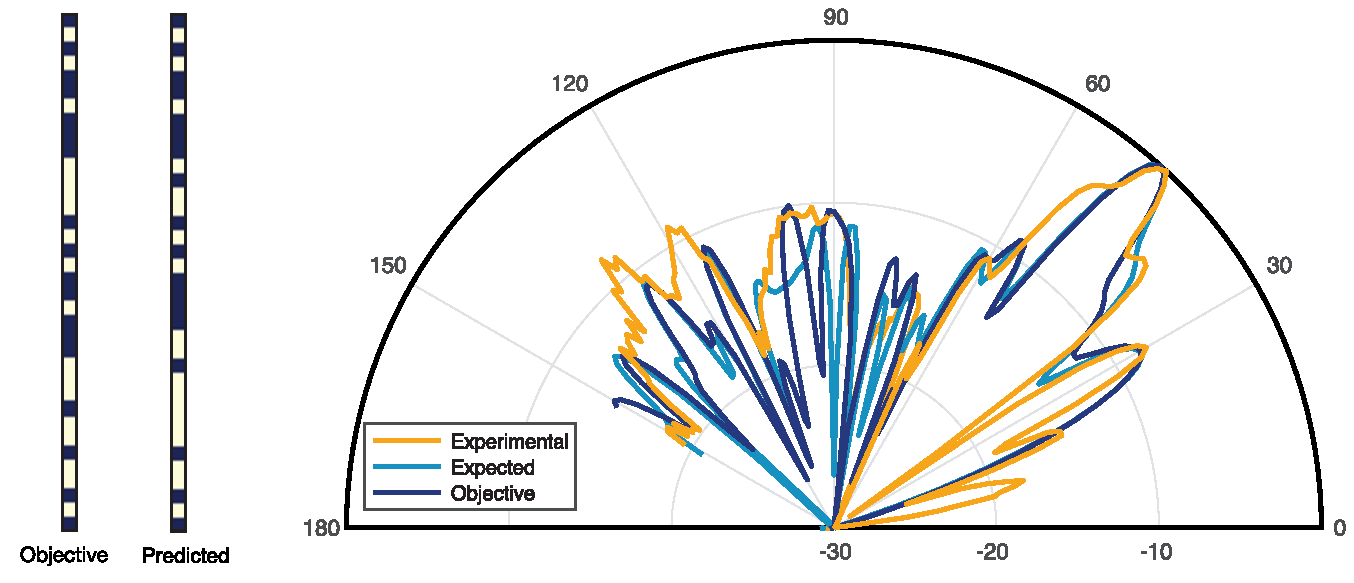
\includegraphics[height=2.1in]{figures/477exppdf2}
	\caption{Comparison of experimental and numerical results for non-uniform periodic slot. The experimental signal is what was measured for the given slot using TDS, the expected is what we expect for the antenna geometry the model predicts, and the objective is the desired signal.}
\end{figure}

\noindent We draw two primary conclusions from Figure 8, which are generated from the model's predictions for low values of MSE. First, the slot predicted by the model predicts a far-field signal quite similar to the objective function. Secondly, the experimental data generally agrees with the simulation data, particularly near the largest peaks, there are certainly differences between the numerical and experimental values. One possible cause is due to the relatively simple setup we are using to measure experimental data and the resulting geometrical difficulties of picking up back-scattering. However, the experimental measurements serve as a satisfactory proof of concept of our model and its usefulness with rapid prototyping techniques like hot stamping when designing antennas. 

\subsection*{Grey Sub-Slot Scheme}

\noindent This more advanced schema significantly expands the scope of the problem because each sub-slot can take one of three values instead of just two: 0\% transparent (i.e. fully metallic), 50\% transparent, and 100\% transparent. We again generate approximately 20,000 samples using numerical simulation where each sub-slot can take on these values using a transition boundary layer. This significantly increases the number of degrees of freedom within the model, which we would expect would allow us to generate slots for a wider array of potential signals.  This is suggested by Figure 9b below; the range of values at each peak is broader in the grey model than for the binary model.
%
\begin{figure}[H]
	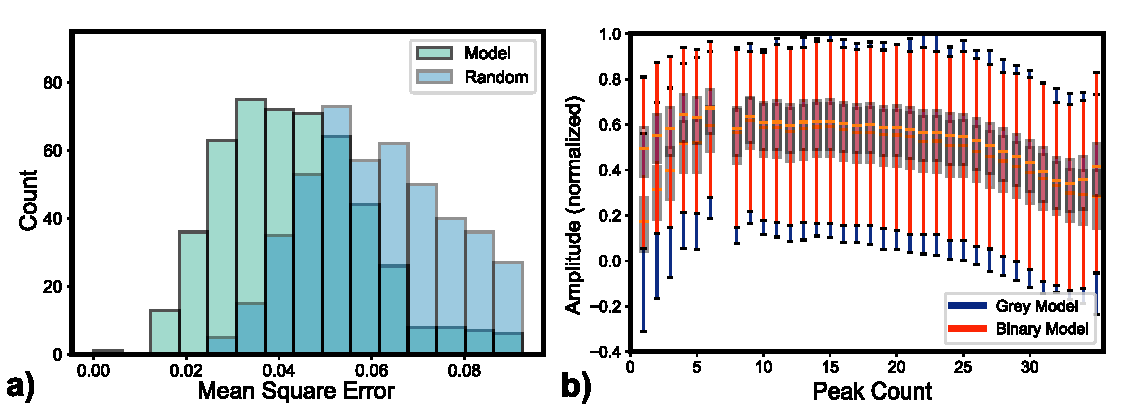
\includegraphics[width=6.5in]{figures/histandboxgreyoverlay}
		\caption{a) The mean square error histogram for both the grey model performance and a control sample. The horizontal offset indicates the model's predictive value and is confirmed by a Z-test. b) A box plot of possible normalized power values for both models. The grey model allows for a wider array of values, as we expect from the increase degrees of freedom in this model.}
\end{figure}

\noindent As with the binary case, we plot a histogram of the model results in Figure 9a and again note the horizontal offset between the model and control. We again conducted two-sided z-test between two samples with the same justifications and again establish a statistically significant difference with p-value of 1.86e-72, indicating significance at a very low value of $\alpha$ (albeit the p-value here is higher than for the binary model, although both are very lower). The average MSE is 0.0434, which is higher than in the binary case, and the sub-slot accuracy is 48.1\%; while higher than the base 33.3\% one would expect given there is a 1/3 chance of correctly guessing, this accuracy is lower than in the binary case. This is not unexpected; due to computational constraints, we generate the same number of training samples as the binary case despite the increased degrees of freedom ($3^{36}$ instead of $2^{36}$, a significant increase). That means in the grey schema, we have a smaller amount of data in relation to the number of possible outcomes, which may explain the decreased accuracy.


\noindent As before, we are interested in comparing the results of our model and numerical simulations to experimental data. However, this is slightly more complicated experimental method -- we need to actually experimentally generate semi-transparent slots. We do this by using the aforementioned hot-stamping technique but instead of using black ink for metallic slots and the absence of ink for transparent slots, we calibrate our TDS system using ``grey'' slots, the idea being that changing the ink color within the greyscale spectrum will directly correlate with the amount of metal deposited on the surface of the antenna. We first calibrate shades of grey with transmission values to determine the greyscale value between 0 and 255 that yields approximately 50\% transmission; we find it to be 109. We then produce our LWAs using the exact same methodology as in the binary case.

\begin{figure}[H]
	\centering
	\includegraphics[height=2.4in]{figures/greyexperiment2}
		\caption{(34 in set). An example of the grey model's performance and comparison to experimental results. The left slot design shows the slot used to produce the objective far-field signal and the right slot design shows the model's prediction. The polar plot shows the far-field signals computed numerically for each of these slots, overlaid with the experimental results collected using TDS. The numerical predicted and objective far-field signals closely agree with an MSE of 0.0311, despite slots that while sharing similarities are somewhat different, and match the experimental data well.}
\end{figure}

\noindent An example of the model's predictive performance is shown in Figure 10, along with a comparison to the experimental results for the predicted slot collected using the method described in the previous paragraph with the TDS setup described in Figure 4c. We draw a handful of conclusions from Figure 10. First, for this example, which has an MSE approximately in the center of the histogram and thus can be considered roughly average performance for the model, the predicted and objective far-field signals generally agree quite well and have very similar shapes, despite having slot patterns that are not exactly the same, as we would expect from Floquet theory -- there are many ways to achieve a linear combination of periodicities. Secondly, the experimental results agree fairly closely with the numerical predicted values. While there are some differences particularly in the backwards direction, it is important to remember that these results were collected using hot-stamping, an inherently inexact rapid-prototyping technique that is particularly imprecise given that we can only generate an approximately 50\% transparent slot subject to the whims of the laster printer, in addiction to the difficulty of measuring back-reflection at large angles $\geq 140$ degrees.  Overall, the experiment confirms the validity of producing LWA metasurfaces in this fashion, and we expect the experimental accuracy to be higher using more advanced methods of producting metasurfaces.

\section*{Conclusion}

\noindent While rapid prototyping methods like hot stamping are useful for quickly testing antenna design, determining how to build an antenna that will produce some given signal is still a work in progress. It is easy to conceive of some far-field signal for some specific purpose (i.e. delivering a signal to receivers at some number of different locations but avoiding eavesdroppers at other locations	) and also to build a prototype of the antenna for rapid experimentation, but the ideas presented here begin to bridge the gap between conception and experimentation. A user with an idea of some highly specific signal might use such a model to obtain a starting point for an antenna geometry, after which techniques like hot-stamping can be used to tweak the antenna until optimal prototype performance is obtained. \\

\noindent There remain many areas of further exploration; we present a baseline model that serves as a proof-of-concept, but it could surely be further improved and optimized by generating more training data and extensively tuning the model hyper-parameters. Additionally, we explore only one additional method of modulation: making some sub-slots partially transparent. It is easy to conceive of other ideas, such as modulating the width of each sub-slot or further increasing the number of intermediate grey steps, all of which serve as significant areas of further research from both modeling and experimental perspectives.

\section*{Data Availability}
The data that support the findings of this study are available from the corresponding author upon reasonable request.

\section*{Code Availability}
The neural network models, analysis, and simulation models are all shared in the public domain at *INSERT REPOSITORY HERE*

\section*{Author Contributions}
J.N. and H.G. conceived the underlying ideas; J.N. built the model, conducted the experiments, analyzed the data, and wrote the text with the assistance of H.G; D.M. supervised the investigation.

\section*{Funding}
This work was supported by the U.S. National Science Foundation?

\section*{Competing Interests}
The authors declare no competing interests. 

\bibliographystyle{plain}
\bibliography{references.bib}
\end{document}
